
\subsection{User-centered Design Method}
\subsubsection{Empathize}
\label{subsec:empathize}
\subsubsection{Define}
\label{subsec:define}

\begin{itemize}
    \item In order to define requirements for the crutches, the range of forces acting on the crutches during use by S1 were determined. The measurements were conducted with the VariLeg II crutches, which are equipped with force sensors. The data can be seen in fig. \ref{fig:forcesensordata}. The evaluation was done for following procedure twice: standing up, sitting down, standing up, walking some steps, sitting down. Peaks were determined to be around 400N. It can also be detected, that for sitting down the pilot loads the crutches with around 200N. The second time sitting down occurs at around 800s, the fourth time around 1150s. The first and third time sitting down can not be recognized due to the lack of reference data. 
\end{itemize}


\begin{figure}
    \centering
    \includegraphics[width=1.8\columnwidth]{Appendix/ergonomic_crutch/forcesensordata.png}
    \onecolumn
    \caption[width=2\columnwidth]{\textbf{Measurements with force sensors:} To determine the load acting on the crutches during standing up, walking and sitting down. The pilot first gets up, sits back down, stands up again, walks some steps and sits back down. This was done twice, during the period from 830s until 890s the measurement was stopped. We can recognize peaks to lie at around 400N}
    \twocolumn
    \label{fig:forcesensordata}
\end{figure}


\subsubsection{Ideate}
\label{subsec:ideate}

\subsubsection{Prototype}
\label{subsec:prototype}

\subsubsection{Evaluate}
\label{subsec:evaluate}
For the evaluation of the different systems custom questionnaires and the system usability scale were used. The summaries of the different forms can be found here:\\
Custom Questionnaires: \textit{i. Ergonomic Crutch Design} \ref{pdf:EFB_EC}, \textit{ii. Length Adjustment Mechanism} \ref{pdf:EFB_LAM}, \textit{iii. Haptic Feedback} \ref{pdf:EFB_HF}, \textit{One Hand Free} \ref{pdf:EFB_OHF}\\
SUS: \textit{i. Ergonomic Crutch Design} \ref{pdf:SUS_EC}, \textit{ii. Length Adjustment Mechanism} \ref{pdf:SUS_LAM}, \textit{iii. Haptic Feedback} \ref{pdf:SUS_HF}, \textit{VariLeg II crutch} \ref{pdf:SUS_VLII}.
\cleardoublepage
\includepdf[pages={1,2,3,4,5}]{Appendix/questionnaire/EFB_crutch_summary.pdf}
\label{pdf:EFB_EC}
\cleardoublepage
\includepdf[pages={1,2,3}]{Appendix/questionnaire/EFB_LAM_Summary.pdf}
\label{pdf:EFB_LAM}
\cleardoublepage
\includepdf[pages={1,2,3}]{Appendix/questionnaire/EFB_HF_Summary.pdf}
\label{pdf:EFB_HF}
\cleardoublepage
\includepdf[pages=1]{Appendix/questionnaire/EFB_OHF_Summary.pdf}
\label{pdf:EFB_OHF}
\cleardoublepage
\includepdf[pages=1]{Appendix/questionnaire/SUS_EC.pdf}
\label{pdf:SUS_EC}
\cleardoublepage
\includepdf[pages=1]{Appendix/questionnaire/SUS_LAM.pdf}
\label{pdf:SUS_LAM}
\cleardoublepage
\includepdf[pages=1]{Appendix/questionnaire/SUS_HF.pdf}
\label{pdf:SUS_HF}
\cleardoublepage
\includepdf[pages=1]{Appendix/questionnaire/SUS_VLII.pdf}
\label{pdf:SUS_VLII}



\begin{enumerate}[i.]
\item{Ergonomic Crutch Design}
\end{enumerate}

During User-Workshops first the requirements were discussed and then designs were established. The users had the possibility to integrate their design wishes into prototypes which were then modelled to achieve the first 3D printed prototype of the control unit.

\begin{figure}
    \centering
    \includegraphics[width=1.0\columnwidth]{Appendix/User-centered_design_method/WS_Werner.jpg}
    \caption{Interviewing the former VariLeg II pilot and current VariLeg enhanced pilot}
    \label{fig:interview}
\end{figure}
\begin{figure}
    \centering
    \includegraphics{Appendix/User-centered_design_method/WS_Rolf.jpg}
    \caption{Workshop environment with the pilots}
    \label{fig:ws_up}
\end{figure}
\begin{figure}
    \centering
    \includegraphics{Appendix/User-centered_design_method/WS_Karton.jpg}
    \caption{Handicrafted control unit design}
    \label{fig:handicraft}
\end{figure}
\begin{figure}
    \centering
    \includegraphics{Appendix/User-centered_design_method/WS_Fimo.jpg}
    \caption{Handicrafted control unit design}
    \label{fig:handicraftfimo}
\end{figure}
\begin{figure}
    \centering
    \includegraphics{Appendix/User-centered_design_method/WS_EKZ.jpg}
    \caption{Discussing the design}
    \label{fig:ekz}
\end{figure}
\cleardoublepage
\label{subsec:Ergonomic Design}

\includepdf[pages=1]{Appendix/ergonomic_crutch/Requirements_ergonomic_crutch.pdf}
\label{subsec:EC requirements}
\includepdf[pages=1]{Appendix/ergonomic_crutch/List_of_different_Modes.pdf}
\label{subsec:list of modes}


\begin{enumerate}[ii.]
\item{Length Adjustment Mechanism}
\end{enumerate}
\label{subsec:LAM}

The length adjustment mechanism had to fulfill many requirements, none of the commercial state-of-the-art solutions fulfilled all the requirments; therefore, a new solution was developed.\\
\begin{figure}
    \centering
    \includegraphics[width=0.8\columnwidth]{Appendix/LAM/3D_prototype_LAM.jpg}
    \caption{The length adjustment mechanism was iteratively designed with 3D prototypes}
    \label{fig:3D_LAM}
\end{figure}
\begin{figure}
    \centering
    \includegraphics[width=0.8\columnwidth]{Appendix/LAM/Zangenassembly.png}
    \caption{The clamp mechanism was designed in CAD.}
    \label{fig:CAD_LAM}
\end{figure}
\begin{figure}
    \centering
    \includegraphics[width=0.8\columnwidth]{Appendix/LAM/bottom_crutch.png}
    \caption{\textbt{The bottom pipe of the crutch:} The bottom part has a slot where a pin can slide along, the feature fulfills two main requirements. The pin indicates the end positions and helps finding the right position for the clamp to snap in. Additionally, the pin prevents the two crutch pipes from turning relative to each other, which would prevent the clamp from snapping in.}
    \label{fig:pin_LAM}
\end{figure}

The mechanism seems very promising, the position of the shoulders of the pilot sitting is more comfortable see fig.\ref{fig:shoulderup} and fig.\ref{fig:shoulderdown}. The pilot can also keep an upright posture despite of uneven grounds, see fig.\ref{fig:tilted}.

\includepdf[pages=1]{Appendix/LAM/requirements_LAM.pdf}
\label{pdf:requirementsLAM}
\includepdf[pages=1]{Appendix/LAM/Auslegung_Druckfeder_V2.pdf}
\label{pdf:spring}



\begin{figure}
    \centering
    \includegraphics[width=1\columnwidth]{Appendix/LAM/tiltedpath.jpeg}
    \caption{The shortened crutch helps the pilot to stand upright on a tilted path despite the difference in height of the ground below the crutches.}
    \label{fig:tilted}
\end{figure}

\begin{figure}
    \centering
    \includegraphics[width=0.8\columnwidth]{Appendix/LAM/shouldersup.JPG}
    \caption{The length adjustment mechanism was iteratively designed with 3D prototypes}
    \label{fig:shoulderup}
\end{figure}

\begin{figure}
    \centering
    \includegraphics[width=0.8\columnwidth]{Appendix/LAM/shouldersdown.JPG}
    \caption{The length adjustment mechanism was iteratively designed with 3D prototypes}
    \label{fig:shoulderdown}
\end{figure}


%%%%%%%%%%%%%%%%%%%%%%%%%%%%%%%%%%%%%%%%%%%%%%%%%%%%%%%%%%%%%%%%%%%%%%%%%%%%%%%%%%%%%%%
\cleardoublepage
\begin{enumerate}[iii.]
\item{Haptic Feedback} 
\end{enumerate}

%%%%%% HF requirements

\includepdf[pages=1]{Appendix/haptic_feedback/requirements_haptic_feedback.pdf}
\label{subsec:HF requirements}
%%%%%% HF Empathize

\includepdf[pages=1]{Appendix/haptic_feedback/Fragen_Thomas_Haptisches_Feedback.pdf}
\label{subsec:HF Vibration}

%%%%%% Schematics of the PCB


\begin{figure}
    \centering
    \includegraphics[width=1\columnwidth]{Appendix/haptic_feedback/Schematics.jpg}
    \caption{\textbf{Schematics of the foot sensor PCB:} The following schematics was used to implement the IEE foot pressure insole in combination witht the ESP32 DevKit V4}
    \label{fig:schematics}
\end{figure}

%%%%%% Integration of the Vibration Motor

\begin{figure}[!t]
	\centering
	\includegraphics[width=1\columnwidth]{Appendix/haptic_feedback/Vibration.jpg}
	\caption{\textbf{Flat Coin Vibration Motor on the inside of the closed cuff}}
	\label{fig: vibration}
\end{figure}


%%%%%% Foot Sensor Placement – Inside the shoe

\begin{figure}[!t]
	\centering
	\includegraphics[width=1\columnwidth]{Appendix/haptic_feedback/Placement_in_Shoe.jpg}
	\caption{\textbf{Placement inside the shoe:} The foot pressure sensor was placed inside the shoe between the inner sole and the outer sole.}
	\label{fig: inside shoe}
\end{figure}

%%%%%% Foot Sensor Placement – Outside the shoe

\begin{figure}[!t]
	\centering
	\includegraphics[width=1\columnwidth]{Appendix/haptic_feedback/Placement_outside_shoe.jpg}
	\caption{\textbf{Placement outside the shoe:} The foot pressure sensor was placed outside the shoe between the outer sole and a self-made sock to avoid the sole from being slippery.}
	\label{fig: oudside shoe}
\end{figure}

%%%%%% Foot Sensor Placement – New shoe attachment

\begin{figure}[!t]
	\centering
	\includegraphics[width=1\columnwidth]{Appendix/haptic_feedback/Aussensohle.JPG}
	\caption{\textbf{New shoe attachment of the VariLeg enhanced exoskeleton:} The soles can be placed on the inside of the new shoe attachment between the pilot's shoe and the new shoe attachment.}
	\label{fig: new shoe attachment}
\end{figure}

%%%%%% Paddings

\begin{figure}[!t]
	\centering
	\includegraphics[width=1\columnwidth]{Appendix/haptic_feedback/Aussensohle.JPG}
	\caption{\textbf{Paddings:} Paddings out of self-adhesive neoprene material was placed on each cell to make sure the force flux runs through the cells. Unfortunately, this led to inner stresses due to bending of the unflexible material.}
	\label{fig: paddings}
\end{figure}

%%%%%% Arduino Nano

\begin{figure}[!t]
	\centering
	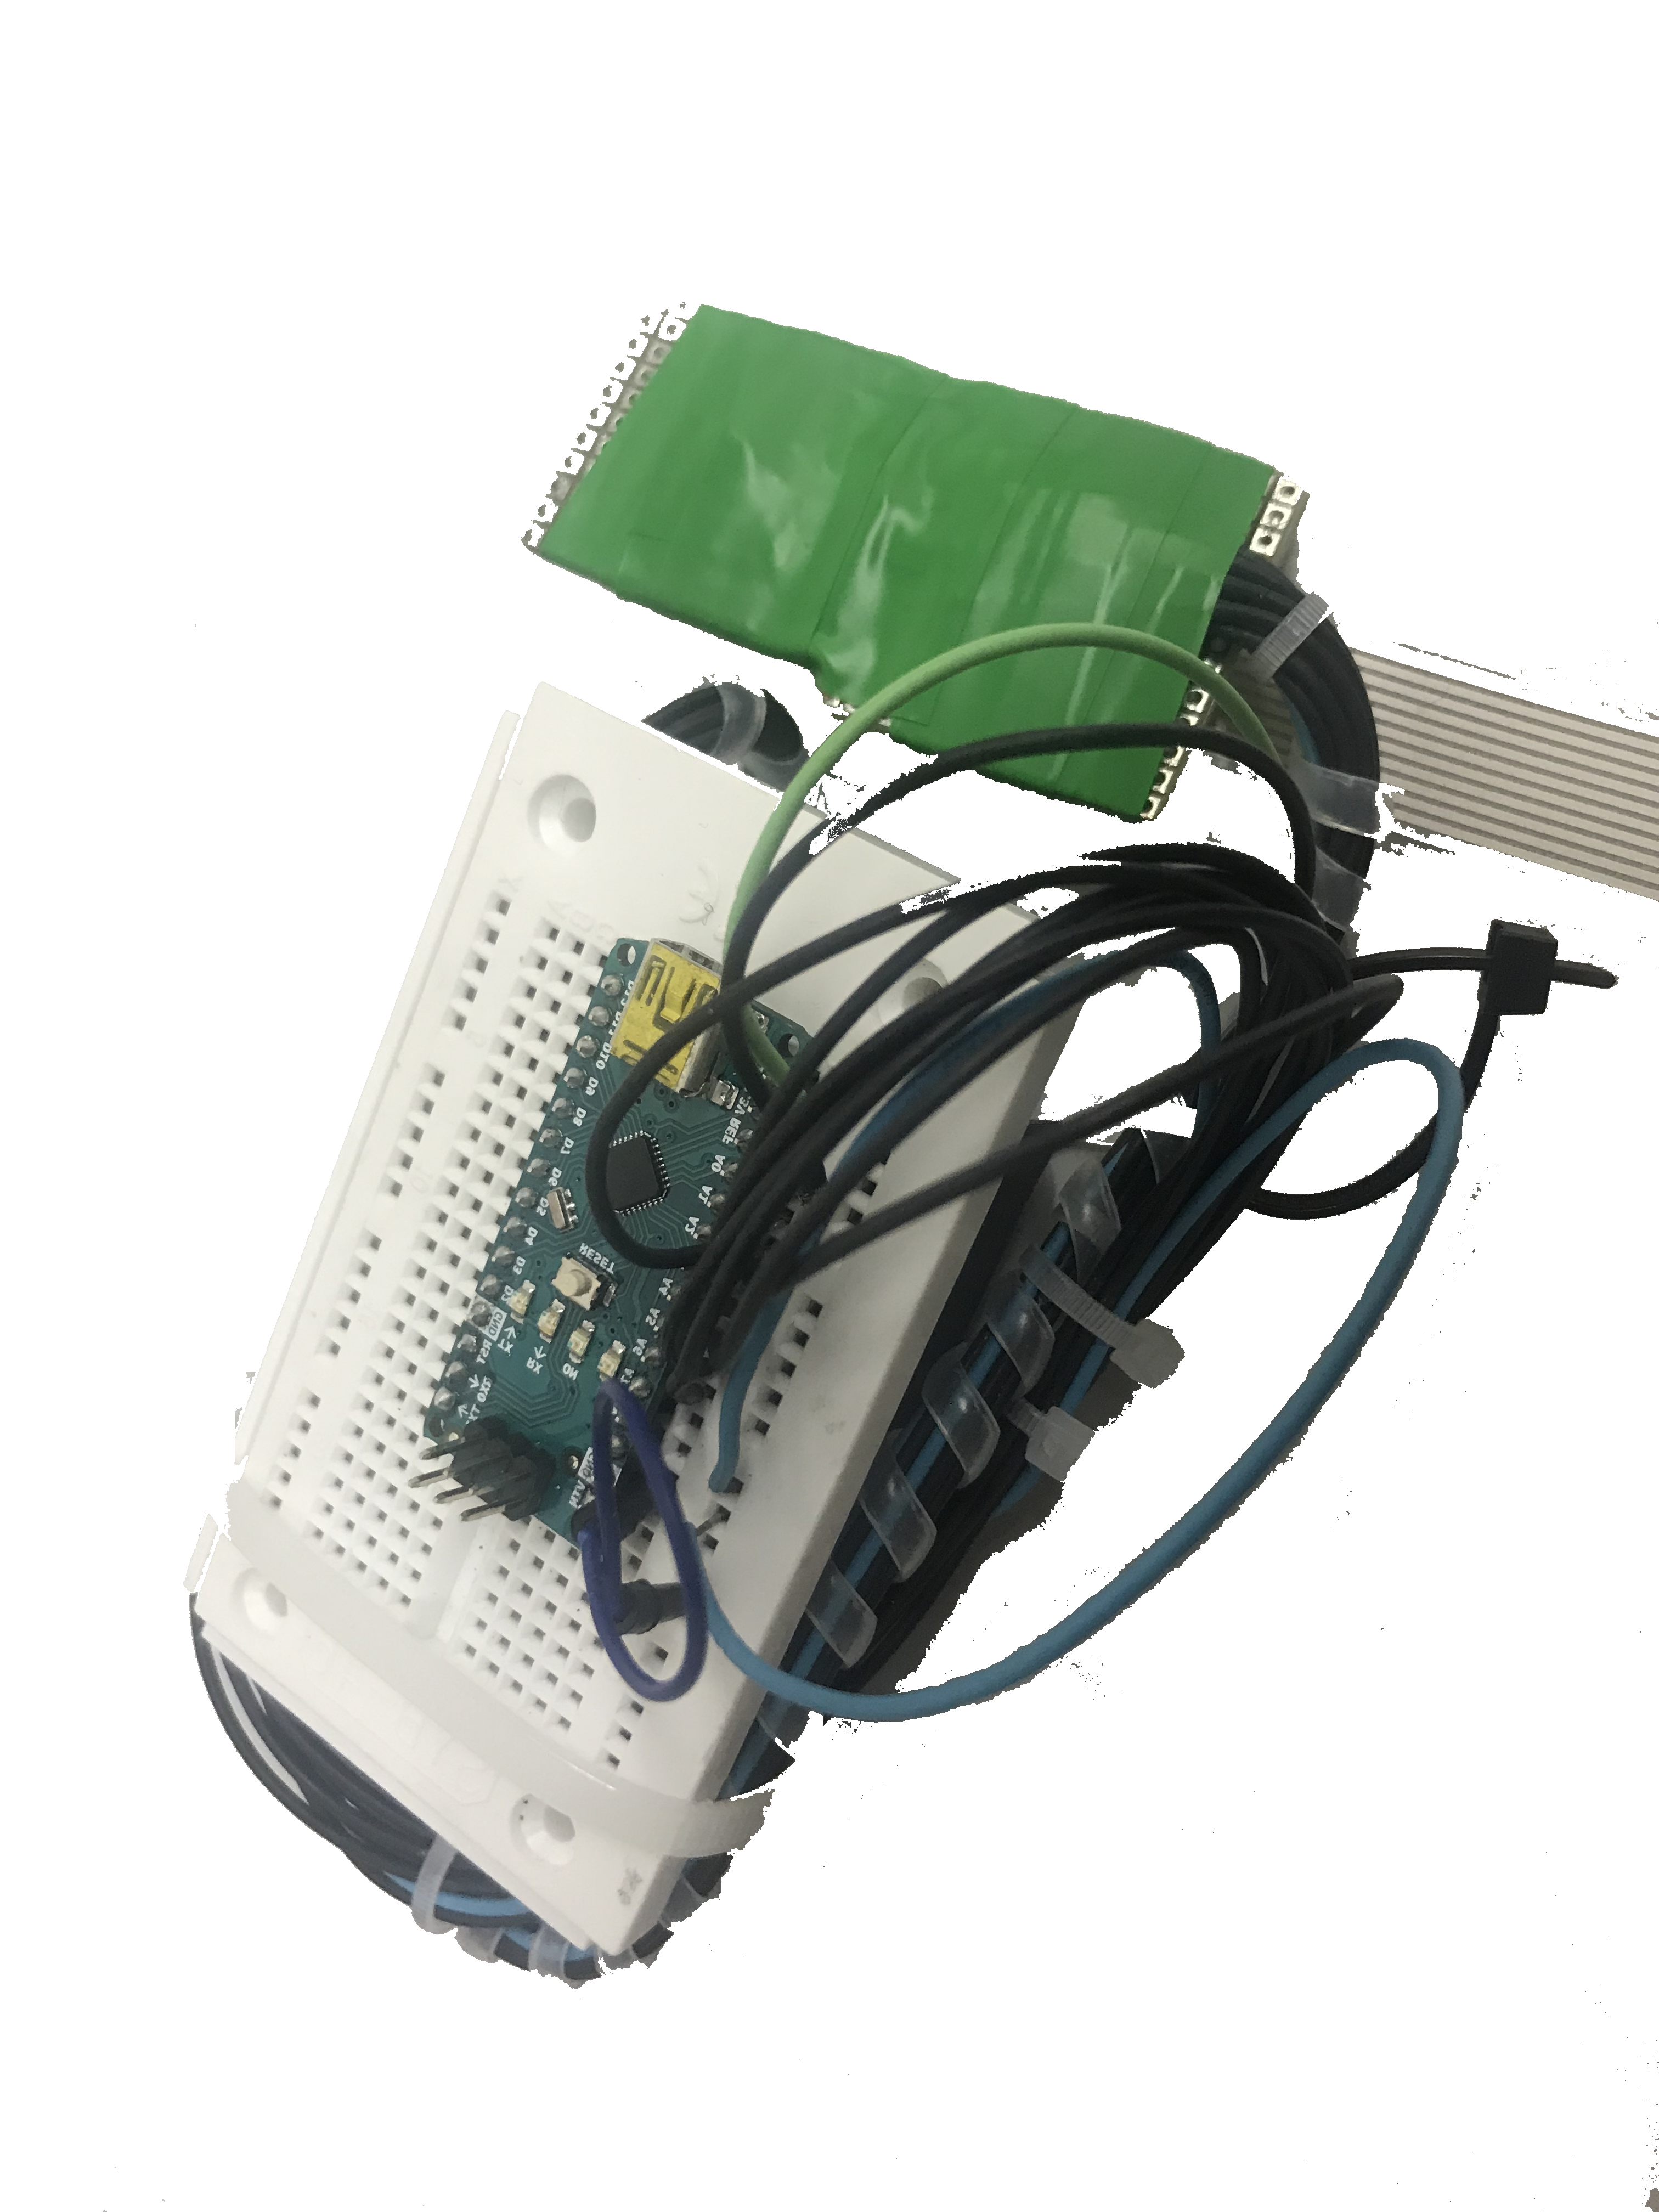
\includegraphics[width=1\columnwidth]{Appendix/haptic_feedback/Setup_mit_arduino.png}
	\caption{\textbf{Initial Setup with a prototype PCB and an Arduino Nano }}
	\label{fig: Arduino Nano}
\end{figure}

%%%%%% PCB selfmade

\begin{figure}[!t]
	\centering
	\includegraphics[width=1\columnwidth]{Appendix/haptic_feedback/handgemachtes_PCB_offen.JPG}
	\caption{\textbf{Prototype PCB}}
	\label{fig: PCB selfmade}
\end{figure}

%%%%%% PCB selfmade

\begin{figure}[!t]
	\centering
	\includegraphics[width=1\columnwidth]{Appendix/haptic_feedback/PCB.JPG}
	\caption{\textbf{Designed PCB:}  This PCB allows the implementation of the foot module compactly in combination with the ESP32 DevKit V4.}
	\label{fig: PCB selfmade}
\end{figure}

%%%%%% Calibration of foot sensor


\begin{table}[!t]
	\renewcommand{\arraystretch}{1.3}
% if using array.sty, it might be a good idea to tweak the value of \extrarowheight as needed to properly center the text within the cells
	\caption{Data of the calibration of the IEE foot sensor by applying aroung 5kg to each sensor cell}
	\label{tab: calibration}
	\centering
% Some packages, such as MDW tools, offer better commands for making tables
% than the plain LaTeX2e tabular which is used here.
		\begin{tabular}{l|ccc}
			\hline
			Sensor Cell Position & Mean [V] & Standard Deviation [V] \\ \hline 
			Heel R  & 0.556 & 0.026  \\
			Heel L  & 0.449 & 0.026  \\
		    Arch & 0.516 & 0.022 \\
			Met 1 & 0.551 & 0.025  \\
			Met 3 & 0.567 & 0.050  \\
			Met 5 & 0.627 & 0.024  \\
		    Hallux & 0.476 & 0.053  \\		    	Toes & 0.466 & 0.029  \\

			\hline
		\end{tabular}
\end{table}

\cleardoublepage
\begin{enumerate}[iv.]
\item{Datasheets} 
\end{enumerate}
%%%%%% Datasheet ESP


\includepdf[pages={1,2,3,4,5,6,7,8,9,10}]{Appendix/haptic_feedback/Datasheet_ESP.pdf}
\label{subsec:HF ESP}

%%%%%% HF Datasheet Insole

\includepdf[page={1,2,3,4,5,6,7,8,9}]{Appendix/haptic_feedback/Datasheet_Insole.pdf}
\label{subsec:HF Insole}

%%%%%% HF Datasheet Flat Coin Vibration Motor


\includepdf[pages={1,2,3,4,5,6,7,8,9,10}]{Appendix/haptic_feedback/Flat_coin_vibration_motor.pdf}
\label{subsec:HF ESP}



%%*************************************************************************

%BEGIN{RELAB} :: optional datasheets and other pdf documents
%\cleardoublepage
%\includepdf[pages={1,3,4-5},angle=0,nup=2x2,frame=true, scale=0.9]{Appendix/PicDatasheet.pdf}
%\includepdf[pages=1]{Appendix/SharpDatasheet.pdf}

%END{RELAB} 

%%*************************************************************************